\section{Proposed Algorithm}
\label{sec:proposed_algorithm}

Throughout the paper, for an $M \times N$ image, we denote $image(a)$ to denote the pixel value of pixel $a$.
We consider binary images i.e. an containing of two types of pixels: object pixel and 
background pixel. Generally, we consider value of object pixel as 1 and value of background pixel as 0. The connected
component labeling problem is to assign a label to each object pixel so that connected object pixels have the same label.
In $2D$ images, there are two ways of defining connectedness: $4$-connectedness and $8$-connectedness. In this paper, we have 
only used the $8$-connectedness of the pixel.


\vspace{3mm}
\subsection{\remsp\ Algorithm}


In the first scan step of \remsp, we process image lines one by one using the
forward scan mask as shown in Figure \ref{fscan1}. We have used the decision 
tree proposed by \cite{Wu2009_LRPC} for determining the provisional label of current pixel
$e$ as we can reduce the number of neighbors using decision tree. Instead of
examining all four neighbors of pixel, say $e$, i.e. $a$, $b$, $c$ and $d$, we only
examine the neighbors according to a desicion tree as shown in Figure \ref{dtree}.
 Let $label$ denote the $2D$ array storing the labels and let $p$ denote equivalence array 
 then according to \lrpc\ algorithm,
three functions used by this decision tree are defined as follows:

$1)$. The one-argument copy function, copy(a), contains one statement:
					$label(e) = p(label(a))$\\
$2)$. The two-argument copy function, copy(c,a), contains one statements:
				$label(e) = merge(p, label(c), label(a))$\\
$3)$. The new label function sets $count$ as $label(e)$, appends $count$ to array $p$, and increments $count$ by $1$.

\begin{figure}
\centering
\begin{tabular}{ | l | c | r | }
 \hline
 a & b & c \\ \hline
 d & e & \multicolumn{1}{r}{} \\ \cline{1-2}
 f & g & \multicolumn{1}{r}{} \\ \cline{1-2}
\end{tabular}
\caption{Forward Scan Mask for \em{ARemSP}}
\label{fscan1}
\end{figure}

\begin{figure}
\centering
\begin{tabular}{ | l | c | r | }
 \hline
 a & b & c \\ \hline
 d & e & \multicolumn{1}{r}{} \\ \cline{1-2}
\end{tabular}
\caption{Forward Scan Mask for \em{RemSP}}
\label{fscan2}
\end{figure}

\begin{figure}
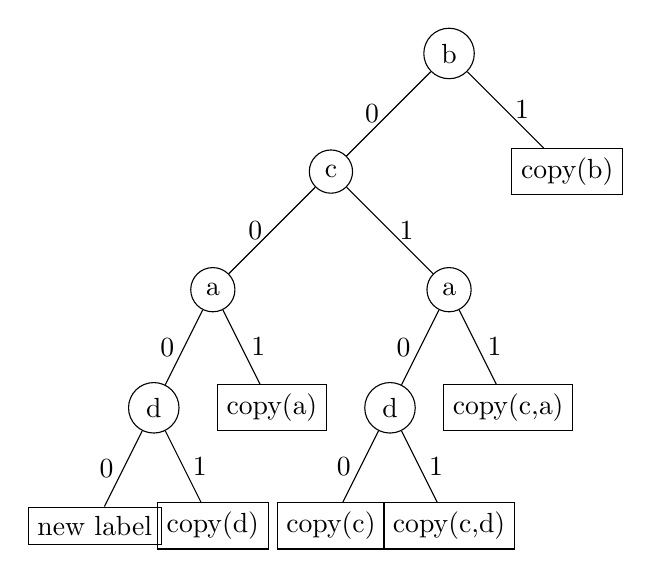
\begin{tikzpicture}[level distance=1.5cm,
  level 1/.style={sibling distance=3 cm},
  level 2/.style={sibling distance=3 cm},
  level 3/.style={sibling distance=1.5cm},
  level 4/.style={sibling distance=1.5cm}]
  \node[circle,draw] {b}
   child 
   {
    	node[circle,draw] {c}
      	child 
      	{
      	    	node[circle,draw] {a}
      	    	child
      	    	{
      	    		node[circle,draw]{d}
      	    		child
      	    		{
      	    			node[rectangle,draw]{new label}
      	    			edge from parent node[left,draw=none] {0}
      	    		}
      	    		child
      	    		{
      	    			node[rectangle,draw]{copy(d)}
      	    			edge from parent node[right,draw=none] {1}
      	    		}
      	    		edge from parent node[left,draw=none] {0}
      	    	}
      	    	child
      	    	{
      	    		node[rectangle,draw]{copy(a)}	
      	    		edge from parent node[right,draw=none] {1}
      	    	}
      	    	edge from parent node[left,draw=none] {0}
      	}
      	child 
      	{
      		node[circle,draw] {a}
      		child
      		{
      			node[circle,draw]{d}
      	    		child
      	    		{
      	    			node[rectangle,draw]{copy(c)}
      	    			edge from parent node[left,draw=none] {0}
      	    		}
      	    		child
      	    		{
      	    			node[rectangle,draw]{copy(c,d)}
      	    			edge from parent node[right,draw=none] {1}
      	    		}
      	    		edge from parent node[left,draw=none] {0}
      		}
      		child
      		{
      			node[rectangle,draw]{copy(c,a)}
      			edge from parent node[right,draw=none] {1}
      		}
      		edge from parent node[right,draw=none] {1}
      	}
      	edge from parent node[left,draw=none] {0}
    }
    child 
    {
    	node[rectangle,draw] {copy(b)}
    	edge from parent node[right,draw=none] {1}
    };
\end{tikzpicture}
\caption{Decision tree for \em{RemSP}}
\label{dtree}
\end{figure}


However, the implementation of \merge\ operation in our proporsed algorithm
\remsp\ is different from that of in \lrpc.\
We have used the implementation of union-find proposed by {\em Rem}
\cite{Patwary2010_RemSP} for merge operation. {\em Rem} integrates the Union
operation with a compression technique known as Splicing $(sp)$. In the case when 
$rootx$ is to be moved to $p(rootx)$ it works as follows: just before this operation, 
$rootx$ is stored in a temporary variable $z$ and 
then, just before moving $rootx$ up to its parent $p(z)$, $p(rootx)$ is set to $p(rooty)$, 
making the subtree rooted at 
$rootx$ a sibling of $rooty$. This neither compromises the increasing parent property (because $p(rootx) < p(rooty)$) 
nor invalidates the set structures (because the two sets will have been merged when the operation ends.) The effect of $sp$
is that each new parent has a higher value than the value of the old parent, thus compressing the tree. The algorithm for
\merge\ is given as Algorithm \ref{alg:merge}. After the first step, we carry
out the analysis phase using \flatten\ algorithm. \flatten\ algorithm also
generates consecutive labels. The algorithm for \flatten\ is given as Algorithm
\ref{alg:flatten}. The full algorithm for \remsp\ is given as Algorithm
\ref{alg:RemSP}. The implementation of $RemSP-I$ is given in Appendix
\ref{appendix}
% \clearpage
\begin{algorithm}[H]
\small
{
	\caption{Pseudo-code for \nremsp\ Scan Phase}
	\label{alg:RemSP-I}
	\textbf{Input:} $2D$ array $image$ containing the pixel values \\
	\textbf{InOut:} $2D$ array $label$ containing the provisional labels and $1D$ array $p$ containing the equivalence info\\
	\textbf{Output:} maximum value of provisional label in $count$
	\begin{algorithmic}[1]
	\Function{Scan\_CCLRemSP}{$image$}
		\For{$row$ in $image$}
			\For{$col$ in $row$}
				\If{$image(e) = 1$}
					\If{$image(b) = 1$}
						\State $copy(b)$
					\Else
						\If{$image(c) = 1$}
							\If{$image(a) = 1$}
								\State $copy(c,a)$
							\Else
								\If{$image(d) = 1$}
									\State $copy(c,d)$
								\Else
									\State $copy(c)$
								\EndIf
							\EndIf
						\Else
							\If{$image(a) = 1$}
								\State $copy(a)$
							\Else
								\If{$image(d) = 1$}
									\State $copy(d)$
								\Else
									\State {\em new label}
								\EndIf
							\EndIf
						\EndIf
					\EndIf
				\EndIf
			\EndFor
		\EndFor
		\State \Return {$count$}
	\EndFunction
	\end{algorithmic}
}	
\end{algorithm}


\begin{algorithm}[H]
\small
{
	\caption{Pseudo-code for RemSP}
	\label{alg:RemSP}
	\textbf{Input:} $2D$ array $image$ containing the pixel values \\
	\textbf{Output:} $2D$ array $label$ containing the final labels
	\begin{algorithmic}[1]
	\Function{RemSP}{$image$}
		\State $RemSP-I(image)$ \Comment{Scan Phase of RemSP}
		\State $flatten(p,count)$ \Comment{Analysis Phase of RemSP}
		\For{$row$ in $image$}  \Comment{Labeling Phase of RemSP}
			\For{$col$ in $row$}
				\State $label(e) \gets p[label(e)]$
			\EndFor
		\EndFor
	\EndFunction
	\end{algorithmic}
}	
\end{algorithm}


\begin{algorithm}[H]
\small
{
	\caption{Pseudo-code for flatten}
	\label{alg:flatten}
	\textbf{InOut:} $1D$ array $p$ containing the equivalance info \\
	\textbf{Input:} Max value of provisional label $count$
	\begin{algorithmic}[1]
	\Function{flatten}{$p$,$count$}
		\State $k \gets 1$
		\For{$i=1$ to $count$}
			\If{$p[i] < i$}
				\State $p[i] \gets p[p[i]]$
			\Else
				\State $p[i] \gets k$
				\State $k++$
			\EndIf
		\EndFor
	\EndFunction
	\end{algorithmic}	
}
\end{algorithm}

\subsection{\aremsp\ Algorithm}


In the first scan step of \aremsp,\ we process image two lines at a time and processes
pixels two by two using the mask shown in figure \ref{fscan2} suggested in \cite{He2012_ARun}. 
We will give the label to both $e$ and $g$ simultaneously. If both $e$ and $g$ are background pixels,
then nothing needs to be done. If $e$ is a foreground pixel and there is no foreground pixel in the mask, we assign a 
new provisional label to $e$ and if $g$ is a foreground pixel, we will give the
label of $e$ to $g$. If there are foreground pixels in the mask, then we assign $e$ any label assigned to 
foreground pixels. In this case, if there is only one connected component in the mask then there is 
no need for label equivalance. Otherwise, if there are more than one connected component in the mask and as 
they are connected to $e$ so all the labels of the connected components are
equivalent labels and needs to be merged. For all the cases, one can refer \cite{He2012_ARun}.
However, our implementation of the union-find is different from \cite{He2012_ARun}.
We use the implementation of union-find proposed by {\em Rem} \cite{Patwary2010_RemSP} for merge operation in
\aremsp.\ We use \flatten\ for analysis phase and generating consequtive
labels.
The full algorithm for \aremsp\ is given as Algorithm \ref{alg:ARemSP}. The
implementation of $RemSP-I$ is given in Appendix \ref{appendix}
\begin{algorithm}[ht]
\small
{
	\caption{Pseudo-code for ARemSP}
	\label{alg:ARemSP}
	\textbf{Input:} $2D$ array $image$ containing the pixel values \\
	\textbf{Output:} $2D$ array $label$ containing the final labels
	\begin{algorithmic}[1]
	\Function{ARemSP}{$image$}
		\State $ARemSP-I(image)$ \Comment{Phase-I of ARemSP}
		\State $flatten(p,count)$ 
		\For{$row$ in $image$}  \Comment{Phase-II of ARemSP}
			\For{$col$ in $row$}
				\State $label(e) \gets p[label(e)]$
			\EndFor
		\EndFor		
	\EndFunction
	\end{algorithmic}	
}
\end{algorithm}


\begin{algorithm}[ht!]
\small
{
	\caption{Pseudo-code for merge\cite{Patwary2010_RemSP}}
	\label{alg:merge}
	\textbf{Input:} $1D$ array $p$ and two nodes $x$ and $y$ \\
	\textbf{Output:} The root of united tree 
	\begin{algorithmic}[1]
	\Function{merge}{$p$,$x$,$y$} 
		\State $root_x \gets x, root_y \gets y$
		\While { $p[root_x] \neq p[root_y]$ }
			\If {$p[root_x] > p[root_y]$}
				\If { $root_x = p[root_x]$ }
					\State $p[root_x] \gets p[root_y]$
					\State \Return{$p[root_x]$}
				\EndIf
				\State $z \gets p[root_x], p[root_x] \gets p[root_y], root_x \gets z$
			\Else
				\If { $root_y = p[root_y]$ }
					\State $p[root_y] \gets p[root_x]$
					\State \Return{$p[root_x]$}
				\EndIf
				\State $z \gets p[root_y], p[root_y] \gets p[root_x], root_y \gets z$
			\EndIf
		\EndWhile
		\State \Return{$p[root_x]$}
	\EndFunction
	\end{algorithmic}	
}
\end{algorithm}

% \begin{algorithm}[ht!]
\small
{
	\caption{Pseudo-code for ARemSP Scan Phase}
	\label{alg:ARemSP-I}
	\textbf{Input:} $2D$ array $image$ containing the pixel values \\
	\textbf{InOut:} $2D$ array $label$ containing the provisional labels and $1D$ array $p$ containing the equivalence info\\
	\textbf{Output:} maximum value of
	provisional label in $count$
	\begin{algorithmic}[1]
	\Function{Scan\_ARemSP}{$image$}
		\For{$row$ in $image$}
			\For{$col$ in $row$}
				\If{$image(e) = 1$}
					\If{$image(d) = 0$}
						\If{$image(b) = 1$}
							\State $label(e) \gets label(b)$
							\If{$image(f) = 1$}
								\State $merge(p,label(e),label(f))$ 
							\EndIf
						\Else
							\If{$image(f) = 1$}
								\State $label(e) \gets label(f)$
								\If{$image(a) = 1$}
									\State $merge(p,label(a))$
								\EndIf
								\If{$image(c) = 1$}
									\State $merge(p,label(e),label(c))$
								\EndIf
							\Else
								\If{$image(a) = 1$}
									\State $label(e) \gets label(a)$
									\If{$image(c) = 1$}
										\State $merge(p,label(e),label(c))$
									\EndIf
								\Else
									\If{$image(c) = 1$}
										\State $label(e) \gets label(c)$
									\Else
										\State $label(e) \gets count,$
										\State $p[count] \gets count,$
										\State $count++$
									\EndIf
								\EndIf
							\EndIf
						\EndIf
					\Else
						\State $label(e) = label(d)$
						\If{$image(b) = 0$}
							\If{$image(c) = 1$}
								\State $merge(p,label(e),label(c))$
							\EndIf
						\EndIf
					\EndIf
					\If{$image(g) = 1$}
						\State $label(g) \gets label(e)$
					\EndIf
				\Else
					\If{$image(g) = 1$}
						\If{$image(d) = 1$}
							\State $label(g) \gets label(d)$
						\Else
							\If{$image(f) = 1$}
								\State $label(g) \gets label(f)$
							\Else
								\State $label(e) \gets count,$
								\State $p[count] \gets count,$
								\State $count++$
							\EndIf
						\EndIf
					\EndIf
				\EndIf
			\EndFor
		\EndFor
		\State \Return {$count$}
	\EndFunction
	\end{algorithmic}	
}
\end{algorithm}







 
